\section{Long Baseline Neutrino Facility}

\begin{figure}
\caption{Long Beamline Neutrino Facility}
\label{fig:LBNF_overallScheme}
\centering
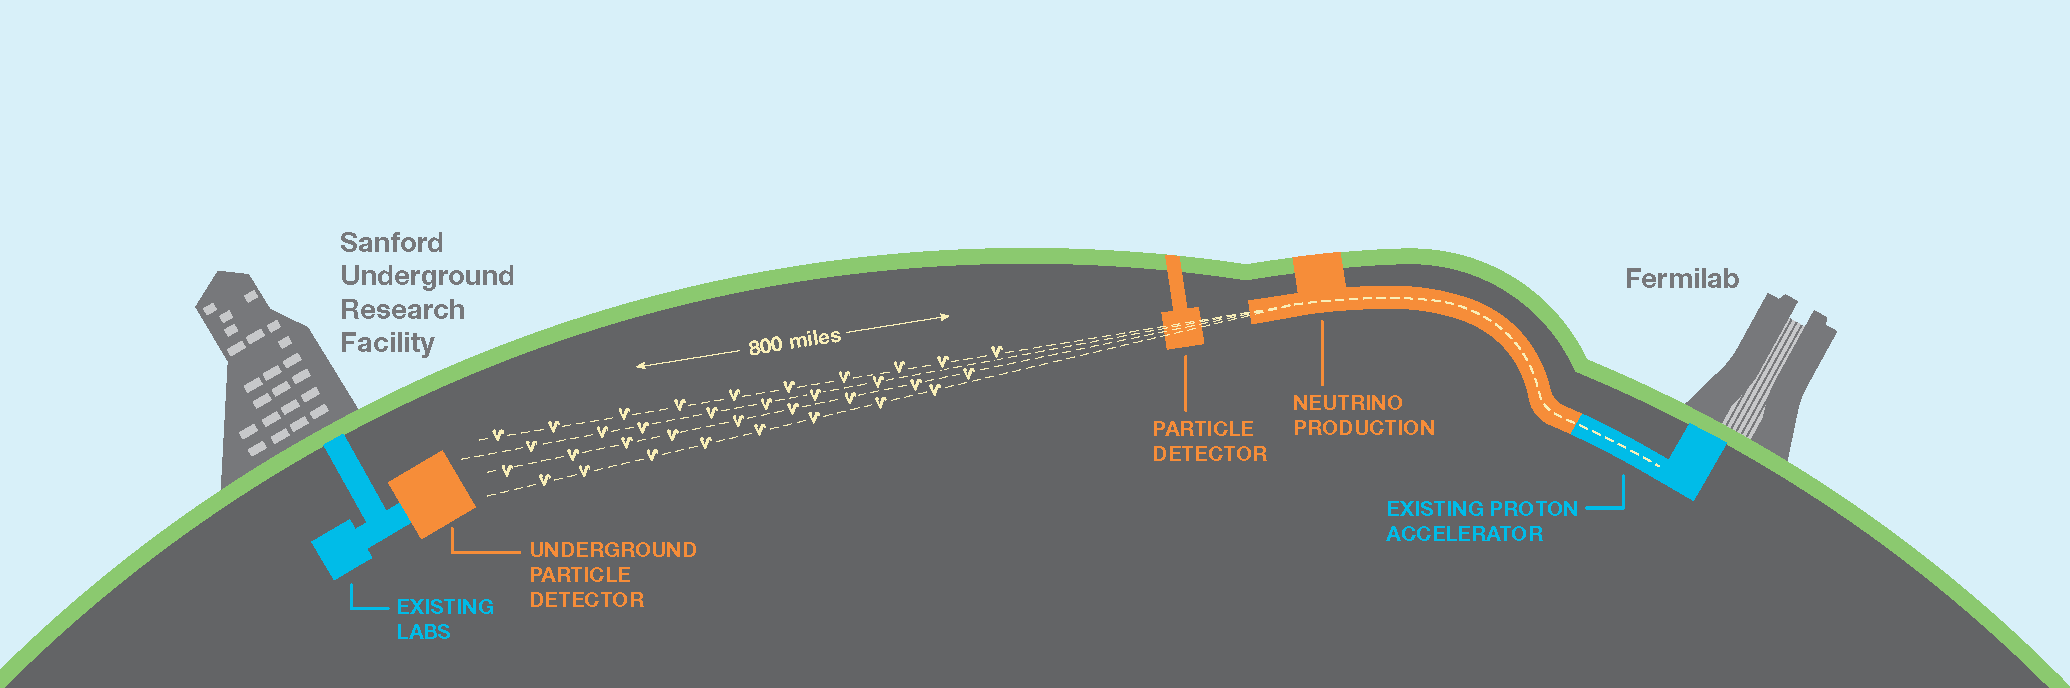
\includegraphics[width=0.95\textwidth, keepaspectratio=true]{figs/LBNF_overallScheme.png}
\\The neutrino flux will be produced using existing proton accelerator in Fermilab. Then neutrinos will be registered by close detector, travel 800 miles through the Earth mantle to the Sanford Underground Research Facility in South Dakota and be registed by far detector. \cite{ref_LBNFweb}   
\end{figure}

\begin{figure}
\caption{Long Beamline Neutrino Facility}
\label{fig:LBNF_nuBeam}
\centering
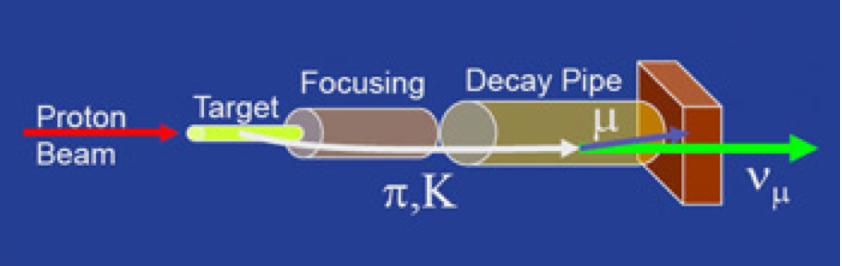
\includegraphics[width=0.35\textwidth, keepaspectratio=true]{figs/LBNF_nuBeam.png}
\\The neutrino beam production at Long Beamline Neutrino Facility. \cite{ref_LBNFweb}   
\end{figure}

The Long Beamline Neutrino Facility is the facility being internationally designed for the future Deep Underground Neutrino Experiment (DUNE) which is going to study neutrino physics. It's going to use the highest intensity neutrino beam ever created. The proton accelerator in Fermilab which was already used in other experiments in Fermilab before will produce the beam of protons. Then protons will hit a target and create kaons and pions through the same reactions as take place in atmosphere when the cosmic protons hit molecules of air.  Pions can be created in the reactions $p+p \rightarrow p+n+\pi^+$, $p+p \rightarrow p+\Delta^{++}+\pi^-$, $p+n \rightarrow p+p+\pi^-$, $p+n \rightarrow n+n+\pi^+$, $p+n \rightarrow p+\Delta^{-}+\pi^+$ etc which go electromagnetically though photon. In more general words, one quark from the accelerator beam proton scatters on the other quark from the proton or neutron of the target substance. They exchange photon which produces quark-antiquark pair. At this moment, the system has seven quarks and one antiquark. The antiquark pairs up with one of the quarks participating in the reaction and the remaining six quarks make two baryons.  The charged pions have formulas $\pi^+ = u\bar{d}$ and $\pi^- = \bar{u}d$ and can be produced with the reactions which only include first generation quarks. The formulas of charged kaons are $K^+ = u\bar{s}$, $K^- = \bar{u}s$. Thus, to produce kaons, the photon has to produce $s\bar{s}$ pair. 
After the mesons are created, neutrinos are produced they go through the focusing camera in decay into the decay pipe as $\pi^+ \rightarrow \mu^+\nu_\mu$, $\pi^- \rightarrow \mu^-\bar{\nu_\mu}$, $K^+ \rightarrow \mu^+\nu_\mu$, $K^- \rightarrow \mu^-\bar{\nu_\mu}$. The branching ratios of charged pions and kaons to decay into $\mu^+\nu_\mu$($\mu^-\bar{\nu_\mu}$) are $(>99.9)\%$ and $(63.55\pm0.011)\%$ respectively.

After being produced in the rections described above, the neutrinos will be detected in the close detector in the Fermilab. Then the neutrinos will travel 800 miles underground and will be detected by Sanford Underground Research Facility in South Dakota.  

\subsection{What questions it's going to answer}
\subsection{How it's going to answer these questions and how it's better  than other experiments}
\subsection{What questions it's not going t oanswer}
